\subsection{IrDA* Infrared Serial Port}

\label{sec:serial_port}

The IrDA port in the {\it \systemNameFull} implements a UART that is connected to the infrared
transmit/receive device on the \DEBoard~board.
This UART is configured for 8-bit data, one stop bit, and no parity, and
operates at a baud rate of 115,200.  The serial port's programming interface 
consists of two 32-bit registers, as illustrated in Figure~\ref{fig:serial_port}. 
The register at address {\sf 0xFF201020} is referred to as the
{\it Data} register, and the register at address {\sf 0xFF201024} is called the {\it
Control} register.

\begin{figure}[h!]
   \begin{center}
       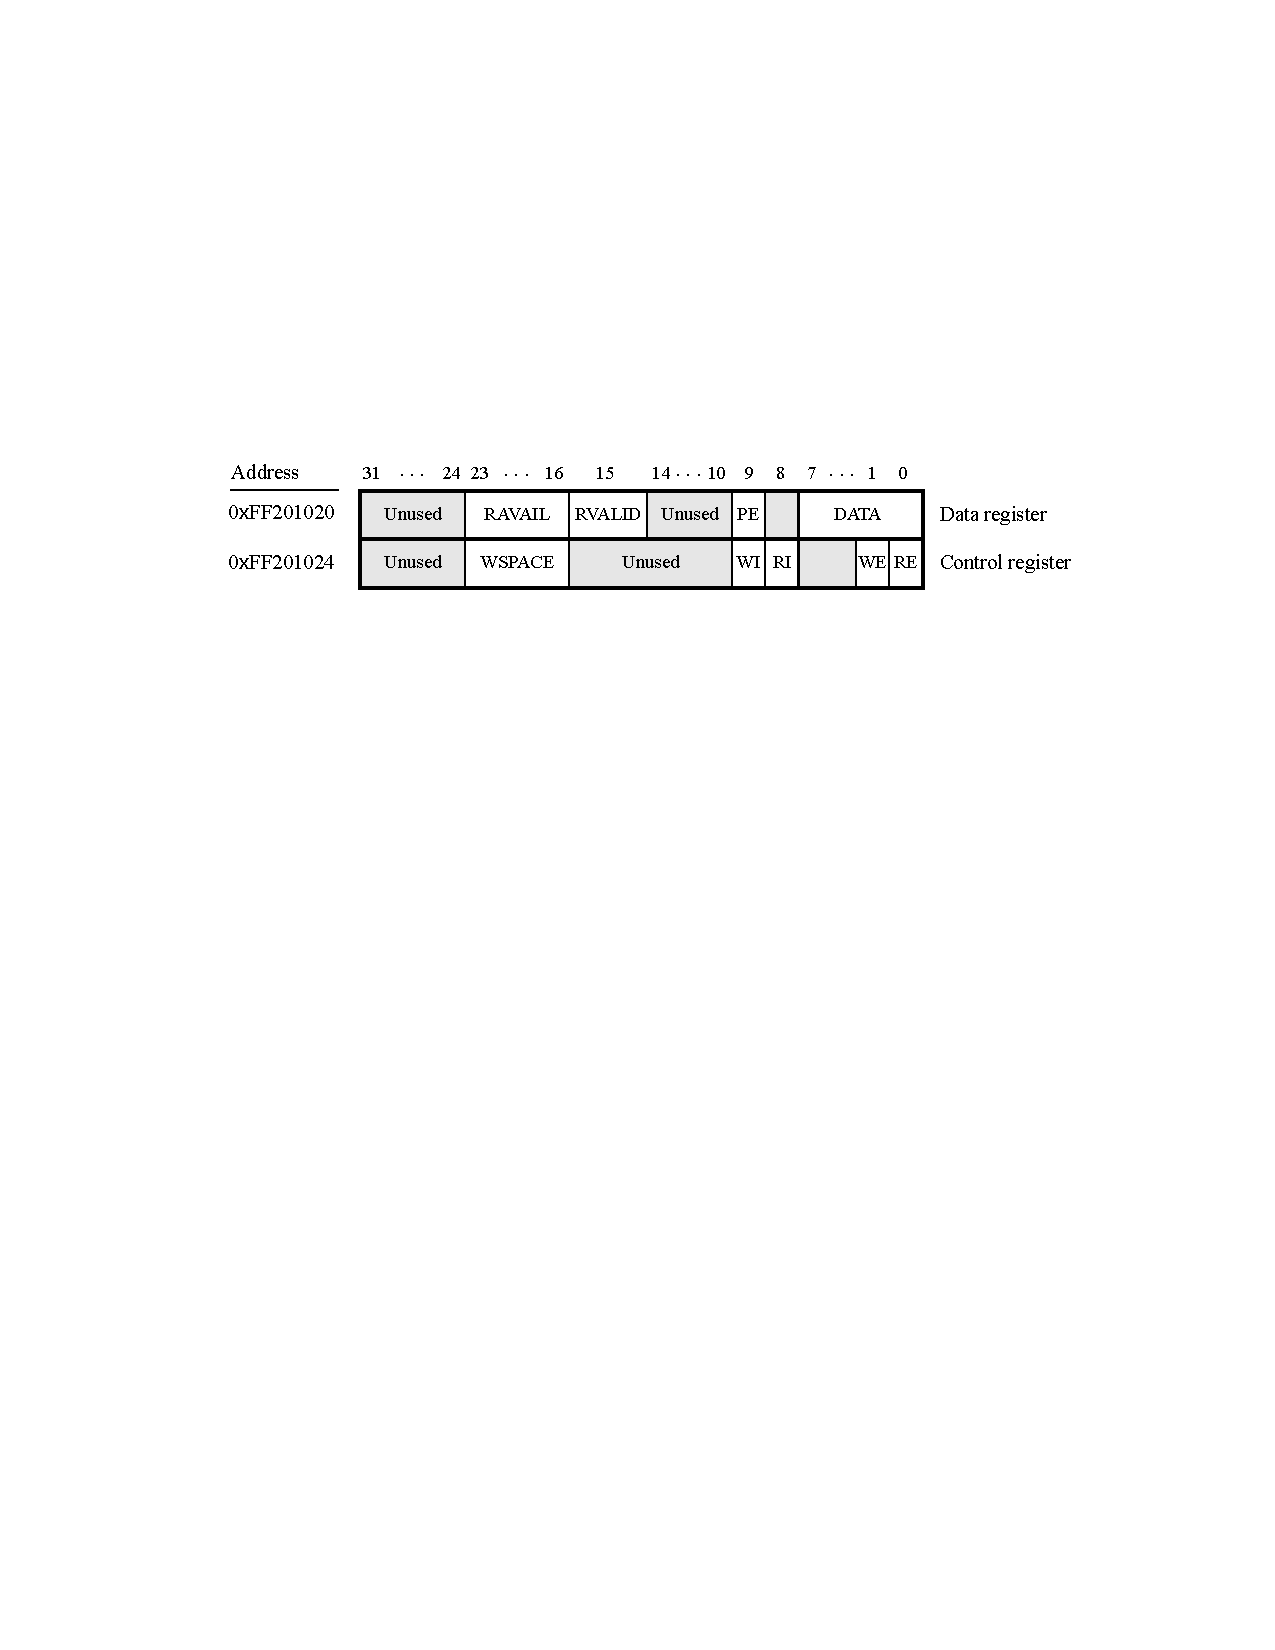
\includegraphics{../../../common/figs/Media_FPGA_IrDA.pdf}
   \end{center}
   \caption{IrDA serial port UART registers.}
	\label{fig:serial_port}
\end{figure}

When character data is received from the IrDA chip it is stored in a 256-character
FIFO in the UART. As illustrated in Figure~\ref{fig:serial_port}, the number 
of characters {\it RAVAIL} currently stored in this FIFO is
provided in bits 23$-$16 of the {\it Data} register.  If the receive FIFO overflows, then
additional data is lost.  When the data that is present in the receive FIFO is available 
for reading, then the value of bit 15, {\it RVALID}, will be 1. Reading the character at
the head of the FIFO, which is provided in bits $7-0$, decrements the value of {\it RAVAIL} 
by one and returns this decremented value as part of the read
operation. If no data is available to be read from the receive FIFO, then {\it RVALID} will 
be set to 0 and the data in bits $7-0$ is undefined.

The UART	also includes a 256-character FIFO that stores data waiting to be sent to the
IrDA device.  Character data is loaded into this register by performing a write to bits 7$-$0
of the {\it Data} register.  Writing into this register has no effect 
on received data.  The amount of space {\it WSPACE} currently available in the transmit FIFO is 
provided in bits 23$-$16 of the {\it Control} register, as indicated 
in Figure~\ref{fig:serial_port}.  If
the transmit FIFO is full, then any additional characters written to the {\it Data} 
register will be lost.

The {\it RE} and {\it WE} bits in the {\it Control} register are used to 
enable \processor~processor interrupts associated with the receive and transmit FIFOs. When enabled, 
interrupts are generated when {\it RAVAIL} for the receive FIFO, or {\it WSPACE} for
the transmit FIFO, exceeds 31. Pending interrupts are indicated in the {\it Control}
register's {\it RI} and {\it WI} bits, and can be cleared by writing or reading data
to/from the UART.


